
\chapter{Digital Television RF Anatomy \& Parametric Beacon Characteristics}
\label{sec:dtv}

\section{Physical Channel Allocations \& the UHF/VHF Raster}
\label{sec:dtv:raster}
In North American broadcast standards (ATSC A/53 \cite{atsc-a53}), Digital Television (DTV) signals are allocated across fixed $B_c = 6\text{ MHz}$ terrestrial frequency channels --- the allocation width inherited from the 1941 monochrome NTSC standard. The telescope observes 400--800~MHz, the octave band set by its 21~cm science goals (mapping neutral hydrogen across redshifts $0.8 \le z \le 2.5$, the epoch in which cosmic expansion transitioned from decelerating to accelerating) and by the electronics economy of second-Nyquist-zone sampling over exactly one octave (an 800~MSPS converter captures 400--800~MHz directly as its own alias, halving the sampling rate otherwise required) \cite{amiri2022chime}. The intersection of this band with the UHF television allocation runs from the 470~MHz band edge --- channel 14, the first UHF assignment, channels 2--13 occupying VHF allocations at 54--88 and 174--216~MHz --- up to 608~MHz (channel 36), the top of the television band after the 2017--2020 incentive-auction repack, bounded above by the internationally protected radio-astronomy allocation at 608--614~MHz (channel 37). The monitored census is therefore $C = 36 - 14 + 1 = 23$ active or incumbent physical DTV channel allocations. Let $c \in \{1, 2, \dots, 23\}$ index the monitored DTV channels. The lower RF boundary of the $c$-th allocation, denoted $f_{\text{edge}}^{(c)}$, is defined by the standard terrestrial UHF television raster: in the core UHF broadcast band (physical channels 14--36), the lower allocation edge for physical channel number $n_{\text{ch}}$ is given analytically in MHz by
\begin{equation}
f_{\text{edge}}(n_{\text{ch}}) = 470 + 6(n_{\text{ch}} - 14) \text{ MHz}.
\end{equation}
Because terrestrial broadcast transmitters emit high Effective Isotropic Radiated Power from elevated horizons, even distant or horizon-diffracted DTV emissions present severe, highly correlated RFI across high-gain astrophysical receiving arrays. This interference environment is directly measured at the site: the telescope's RFI characterization identifies television station bands across 480--580~MHz among the strongest persistent features in its spectrum, alongside intermittent few-second events --- 6~MHz-wide bursts of distant broadcast channels scattered into the beam by meteor ionization trails and aircraft \cite{amiri2022chime}. DTV energy therefore arrives through two distinct modes, persistent carriers on line-of-sight and diffracted paths, and transient scattered bursts; the flagging system of this work must detect both, which shapes the per-frame decision cadence of Chapter~\ref{sec:pipeline}.

\section{8-VSB Signal Anatomy \& the Normative Clock Relations}
\label{sec:dtv:vsb}

An ATSC~A/53 broadcast occupies a $B_c=6$~MHz allocation using eight-level
vestigial-sideband modulation.  The quantities used by the detector come from
two different kinds of statements in the standard, and the distinction matters:
the clock relations are exact, whereas the root-raised-cosine roll-off is a
separately specified nominal response.  Treating those two categories as one exact ``allocation-fill'' identity would impose a relation the standard does not state.

The exact symbol rate is inherited from the 4.5-MHz picture--sound spacing and
the NTSC line-rate relation.  A/53 specifies
\begin{equation}
\label{eq:atsc:symbolrate}
R_s = 684\left(\frac{4.5~\mathrm{MHz}}{286}\right)
    = \frac{1539}{143}~\mathrm{MBd}
    \approx 10.762238~\mathrm{MBd}.
\end{equation}
Equivalently, because $4.5~\mathrm{MHz}=3B_c/4$ for a 6-MHz allocation,
\begin{equation}
R_s=\frac{513}{286}B_c,
\qquad
B_N=\frac{R_s}{2}=\frac{513}{572}B_c
    \approx 5.381119~\mathrm{MHz},
\end{equation}
where $B_N$ is the Nyquist bandwidth associated with the symbol clock.  The
standard's framing hierarchy is synchronized to the same clock: a data segment
contains four segment-sync symbols and 828 data symbols, and the coded payload
carried by those 828 symbols corresponds to one Reed--Solomon-protected
transport packet \cite{atsc-a53}.  These relations establish the exact timing
used by the pilot-frequency calculation below; they do not determine the
spectral roll-off.

A/53 separately specifies a nominal linear-phase transmitter RRC response with
roll-off
\begin{equation}
\alpha=0.1152.
\end{equation}
The concatenated transmitter and receiver responses are therefore nominally a
raised cosine.  Using the exact $B_N$ above gives
$B_N(1+\alpha)\approx6.001024$~MHz.  The approximately 1-kHz difference from
6~MHz is not a physical excess to be explained by a new constraint; it is the
consequence of combining an exact clock with a nominal roll-off quoted to four
decimal places.  The standard itself depicts the channel occupancy at rounded
scales of 5.38~MHz and 0.31-MHz transition regions \cite{atsc-a53}.  The
transmission mask, not an inferred rational value of $\alpha$, is the regulatory
boundary.  No later detector calculation depends on the skirts filling the
allocation exactly.

The data stream is randomized, error-corrected, interleaved, and trellis-coded
before mapping to levels $\{\pm1,\pm3,\pm5,\pm7\}$.  In a narrow spectrometer
cell and over the short frame used here, the resulting payload is therefore
well approximated as broadband noise-like power, although it is not
mathematically Gaussian and the standard also contains deterministic segment-
and field-synchronization sequences.  Those qualifications are important for
claims about alternative detectors.  They do not change the narrower design
fact used here: the continuously present pilot concentrates coherent energy far
more strongly in frequency than either the randomized payload or the distributed
synchronization structure.

\section{The Suppressed-Carrier Pilot as a Detection Beacon}
\label{sec:dtv:pilot}

A/53 inserts a small in-phase pilot at the suppressed-carrier frequency,
describing its position nominally as 309~kHz above the lower band edge and
providing an exact frequency relation in the accompanying note
\cite{atsc-a53}.  Expressed through the exact symbol rate, that relation is
\begin{equation}
\label{eq:pilotoffset}
\Delta f_{\mathrm{pilot}}
 = \frac{B_c}{2}-\frac{R_s}{4}
 = B_c\left(\frac{1}{2}-\frac{513}{1144}\right)
 = \frac{59}{1144}B_c
 = \frac{177}{572}~\mathrm{MHz}
 \approx 309.440559~\mathrm{kHz}.
\end{equation}
For physical channel $c$,
\begin{equation}
\label{eq:pilotfreq}
f_{\mathrm{pilot}}^{(c)}
 = f_{\mathrm{edge}}^{(c)}+\frac{177}{572}~\mathrm{MHz}.
\end{equation}
The weight generator stores this offset rounded to the hertz,
309.441~kHz.  The resulting 0.44-Hz representation error is far below the
11.9-Hz fine-bin spacing and is absorbed by the per-channel anchor measured from
the survey.

The exact frequency relation should not be confused with an exact roll-off
identity.  Under the independently specified nominal $\alpha=0.1152$, the
half-amplitude point of the lower composite raised-cosine transition lies at
approximately 309.95~kHz.  The pilot is therefore close to that point, as the
standard's rounded 0.31-MHz drawing suggests, but not exactly fixed to it by the
same rational integer.  Figure~\ref{fig:vsb} makes the distinction visible.

\begin{figure}[t]
\centering
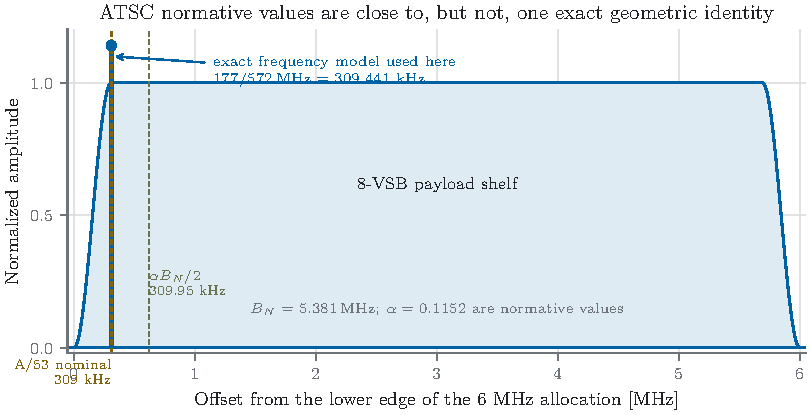
\includegraphics[width=0.98\linewidth]{figs/fig_vsb_standard_model.pdf}
\caption[ATSC pilot frequency and nominal roll-off]{ATSC~A/53 normative values and the near-coincidence that must not be promoted to an exact identity. The standard's exact pilot-frequency relation gives 309.441~kHz above the lower allocation edge (nominally 309~kHz), while the half-amplitude point implied by the separately specified nominal roll-off $\alpha=0.1152$ lies near 309.95~kHz. The ${\sim}0.51$-kHz separation is negligible for the detector's measured-anchor strategy but invalidates the earlier claim that the pilot is exactly the $-6$-dB point because of a common integer factor. The spectral envelope is schematic; the regulatory transmission mask is the governing boundary.}
\label{fig:vsb}
\end{figure}

The pilot is synthesized by adding a DC level 1.25 to every composite symbol
(data and synchronization) before suppressed-carrier modulation.  For the
nominal equiprobable eight-level data model,
$\langle a_n^2\rangle=21$, so the pilot-to-data power ratio is
\begin{equation}
\frac{P_{\mathrm{pilot}}}{P_{\mathrm{data}}}
 = \frac{1.25^2}{21}
 = \frac{25}{336}
 \approx 0.0744,
\end{equation}
consistent with the standard's statement that the pilot is approximately
11.3~dB below the average data signal power \cite{atsc-a53}.  This is a nominal
mean-power relation, not a statement that an arbitrary received 6-MHz spectrum
must reproduce the ratio without scatter.

The corresponding transmitter-side proxy is
\begin{equation}
\label{eq:shelfproxy}
P_{\mathrm{data}} = \frac{336}{25}P_{\mathrm{pilot}},
\qquad
S_{\mathrm{shelf}} \approx
\frac{336}{25}\frac{P_{\mathrm{pilot}}}{B_N},
\end{equation}
where the second expression adopts a flat-shelf approximation over the Nyquist
band.  Concentrating the pilot power in a spectral line gives it roughly
56~dB more power spectral density than the payload per hertz.  That
concentration, continuous presence while the transmitter radiates, and nominal
frequency standardization make it the appropriate low-cost beacon for this
work.

Equation~\eqref{eq:shelfproxy} is the starting model for the word
``proxy,'' not its validation.  Frequency-selective propagation, transmitter
filtering, and the receiver bandpass can change the received pilot-to-shelf
ratio across a 6-MHz allocation.  The archive products used here observe only
the pilot-containing coarse channel and therefore cannot measure that transfer.
Chapter~\ref{sec:bao} carries it explicitly as a conditional model, and
Chapters~\ref{sec:survey} and \ref{sec:calibration} specify the simultaneous
across-allocation spectra required to turn it into a measured distribution.
The matched-filter optimality statement is likewise limited to the declared
known-tone Gaussian model; the complete calibrated detector and competing
cyclostationary or decoding-assisted methods remain empirical comparisons.

\section{The Transmitter Population \& the Propagation Environment}
\label{sec:dtv:environment}

Equation~\eqref{eq:pilotfreq} fixes where a pilot \emph{should} be; what stands behind the phrase ``to within transmitter tolerance'' is a population, and its structure turns out to matter as much as the standard itself. The population has two tiers, and the regulatory record explains why. Full-service (``primary'') stations are high-power facilities whose analog-era rule held the visual carrier to $\pm 1$~kHz \cite{cfr2015tv}, and whose co-channel coordination practice --- precise frequency offsets negotiated so that mutual interference between high-power neighbors interleaves rather than beats --- holds them to tens of hertz in practice: the discipline is enforced less by rule than by the mutual protection of stations that can hurt each other. Translators, boosters, and low-power stations (``secondary'' services under Part~74) are rebroadcast relays filling terrain shadows, historically licensed under tolerances orders of magnitude looser and typically built on aging or low-cost frequency synthesis; they protect full-service stations by displacement, not by precision, so nothing in their operating economics rewards a disciplined carrier. The current rules sharpen this asymmetry to its logical endpoint: today's \S 73.1545 assigns carrier departure tolerances to AM, FM, and international stations only --- television is absent from the list --- and the Part~74 tolerance section, \S 74.761, is \emph{[Reserved]}: deleted \cite{cfr731545,cfr74761}. Frequency discipline in the modern DTV band is therefore a matter of coordination incentive rather than regulation, and the incentive binds exactly one tier. The expected offset population is a tight core of disciplined primaries surrounded by a broad skirt of undisciplined secondaries.

That expectation was first explored because the detector's window geometry depends on it. A preliminary regional station-list summary was assembled from the RabbitEars master compilation of the FCC's Licensing and Management System and ISED Canada's spectrum authorizations, with each entry's service class and compiled distance to the site. The summary contains $132$ records across the DTV band within $500$ miles: $49$ full-service primaries and $83$ secondaries --- \emph{sixty-three percent of that historical list is the undisciplined tier} --- and Table~\ref{tab:census} preserves its first-measured ten-channel reduction. Its counts and distances pre-date the current ISED overlay and are retained as a legacy analysis input, not as current licensed-site adjudications. For mapping, the reproducible PilotProxy reduction combines the reported-on-air ATSC~1.0 and physical-channel normalization with the ISED licence overlay: it expands multi-channel facilities, merges shared physical carriers, and retains the overlay's licence-only candidates in an inclusive $499$-row envelope at $162$ distinct source range--bearing sites. The ISED overlay then adjudicates every Canadian row for which a current licence match was established: matched rows take the licensed transmitter site --- the compilation had anchored several entries on the community instead, and nearest to the telescope the Penticton channel-30 rebroadcaster CHKL-1 stands at $37.8$~km, not the compiled $17.7$~km, in agreement with the archived RabbitEars study printout --- two relays with no current licence are dropped, nine analog-listed low-power stations holding digital licences enter, and every matched row carries the licensed effective radiated power. Rows without a licence match remain explicitly unverified rather than inheriting that adjudication. The two products answer different questions and are not interchangeable. Figure~\ref{fig:census:map} therefore shows the inclusive normalized $500$-mile envelope while retaining the individual-record $120$-mile detail. The population's spectral face is measured independently from the survey products themselves: each product stores the archive-averaged $16384$-point spectrum of its coarse channel, and Figure~\ref{fig:census:psd} plots that average around each pilot. The channels sort into two clear morphologies. Where the local field is quiet, the average is a compact cluster --- at most a resolved companion or shoulder inside the fine span and an isolated narrow line or two beyond it (channels 27, 28, 29, 34, 36; channel 29's cluster rides on a visibly tilted baseline, the odd-order structure the symmetric reference pair of Chapter~\ref{sec:param} cancels exactly). Where the field is crowded, a \emph{main lobe} at the dominant transmitter's offset stands over a resolved \emph{forest of sidelobes} spanning several kilohertz (channels 30, 31, 32). The narrow, stable multiplicity is consistent with the surrounding transmitter population and is not well described as a single carrier undergoing a time-varying Doppler smear; the inclusive census alone, however, does not identify which listed emitters produced a particular spectral line.

The current census envelope and spectra show why a simple proximity ranking is not a defensible propagation model. Channel 30, whose shelf sits at system noise and is the loudest measured, does have the licence-matched CHKL-1 relay only $37.8$~km away. But channel 27 is masked above $98\%$ even though its nearest current envelope row is the reported-on-air but licence-unverified K27OO-D at $267.2$~km; channel 33 has 15 envelope rows, not the legacy table's three, with the nearest a reported-on-air but licence-unverified translator at $101.4$~km; and channel 36's nearest envelope row is likewise unverified at $135.2$~km. Those rows constrain geometric plausibility but neither prove reception nor attribute occupancy to a transmitter. The survey-measured anchors remain the defensible evidence --- per-channel residuals of hundreds of hertz to $1.4$~kHz, stable within eras, and stepping when the dominant spectral component changes (Section~\ref{sec:bao:eras}). Channel 33's averaged spectrum is \emph{dominated} by a component at its own offset, ${\approx}3.6$~kHz below the synthesized pilot and standing $16$~dB over the lobe at the pilot position in the archive average, which is the measured origin of the spread-across-schedules fine structure that its wide-null diagnosis chases (Section~\ref{sec:bao:verdicts}). It is the observed spectral spread, together with the population envelope and its explicit evidence limits, that sizes the analysis window of Section~\ref{sec:param:tradeoffs}; the census is not used here as a propagation measurement.

The normalized census is deliberately a conservative maximum envelope rather
than a list of 499 observed carriers.  Its frozen input preserves the
\texttt{dtv\_transmitter\_census\_v1} schema and a per-row evidence state: 421
records were reported on air but await licence verification, 67 were reported
on air and licence-matched, and 11 are licence-only candidates whose emission
was not confirmed.  Figure~\ref{fig:census:map} includes that envelope for
geometric context; the evidence labels prevent licence-only candidates from
being promoted to detections.

\begin{table}[t]
\centering
\caption[Legacy 132-record station-list summary for the first-measured ten channels.]{The legacy 132-record regional station-list summary used during the first-measured analysis: records per physical channel, split by service tier (full-service primaries versus the translator/rebroadcaster/low-power secondary tier), with each channel's nearest facility as recorded in that compilation. The counts and distances pre-date the current ISED re-siting and are preserved for auditability; they are not current licensed-site claims and are not used for the quantitative proximity discussion above. Across channels 14--36, the historical summary contains 49 primary and 83 secondary records. It is distinct from the current normalized 499-row envelope used by Figure~\ref{fig:census:map}.}
\label{tab:census}
\begin{tabular}{lccccl}
\toprule
 & facilities & primary & secondary & \multicolumn{2}{l}{nearest facility} \\
\midrule
ch\,27 & 6 & 2 & 4 & CHBC-DT (pri.) & $60$~km \\
ch\,28 & 5 & 2 & 3 & CH5533-DT (sec.) & $130$~km \\
ch\,29 & 6 & 2 & 4 & K29ED-D (sec.) & $401$~km \\
ch\,30 & 8 & 2 & 6 & CHKL-1 (sec.) & in Penticton \\
ch\,31 & 7 & 1 & 6 & CH4491-DT (sec.) & $60$~km \\
ch\,32 & 7 & 3 & 4 & CH5534-DT (sec.) & $130$~km \\
ch\,33 & 3 & 3 & 0 & CKVU-DT (pri.) & $241$~km \\
ch\,34 & 6 & 2 & 4 & CH4490-DT (sec.) & $60$~km \\
ch\,35 & 5 & 2 & 3 & CBUT-DT (pri.) & $242$~km \\
ch\,36 & 4 & 1 & 3 & KZJO (pri.) & $277$~km \\
\bottomrule
\end{tabular}
\end{table}

\begin{figure}[t]
\centering
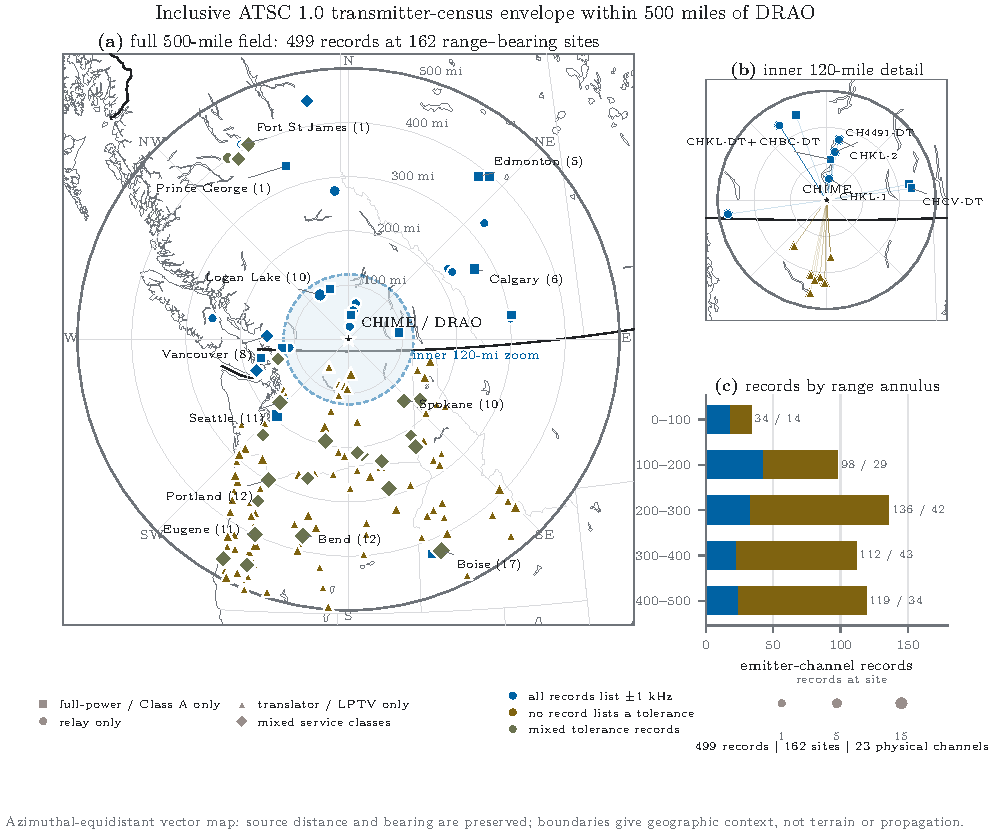
\includegraphics[height=0.68\textheight,width=0.98\linewidth,keepaspectratio]{figs/fig_census_map.pdf}
\caption[Conservative 500-mile DTV transmitter census envelope]{The normalized transmitter-census maximum envelope within $500$ miles of DRAO. \textbf{(a)} The inclusive export contains 499 emitter-channel records at 162 distinct source range--bearing sites; exactly coincident records are aggregated for legibility, with marker area retaining their multiplicity. The frozen rows preserve the evidence split (421 reported-on-air/unverified, 67 reported-on-air/licence-matched, and 11 licence-only candidates), so inclusion on the map is not a claim that a carrier was observed. Shape records the site's service-class composition and color records whether its entries list a $\pm1$~kHz transmitter-frequency tolerance. \textbf{(b)} The inner $120$-mile individual-record detail preserves the view used to diagnose the nearby field. \textbf{(c)} Emitter-channel records by $100$-mile annulus; annotations give records/sites. The DRAO-centred azimuthal-equidistant vector map preserves the supplied distances and bearings. Coastlines and administrative boundaries provide geographic context but intentionally do not imply terrain screening or propagation.}
\label{fig:census:map}
\end{figure}

\begin{figure}[t]
\centering
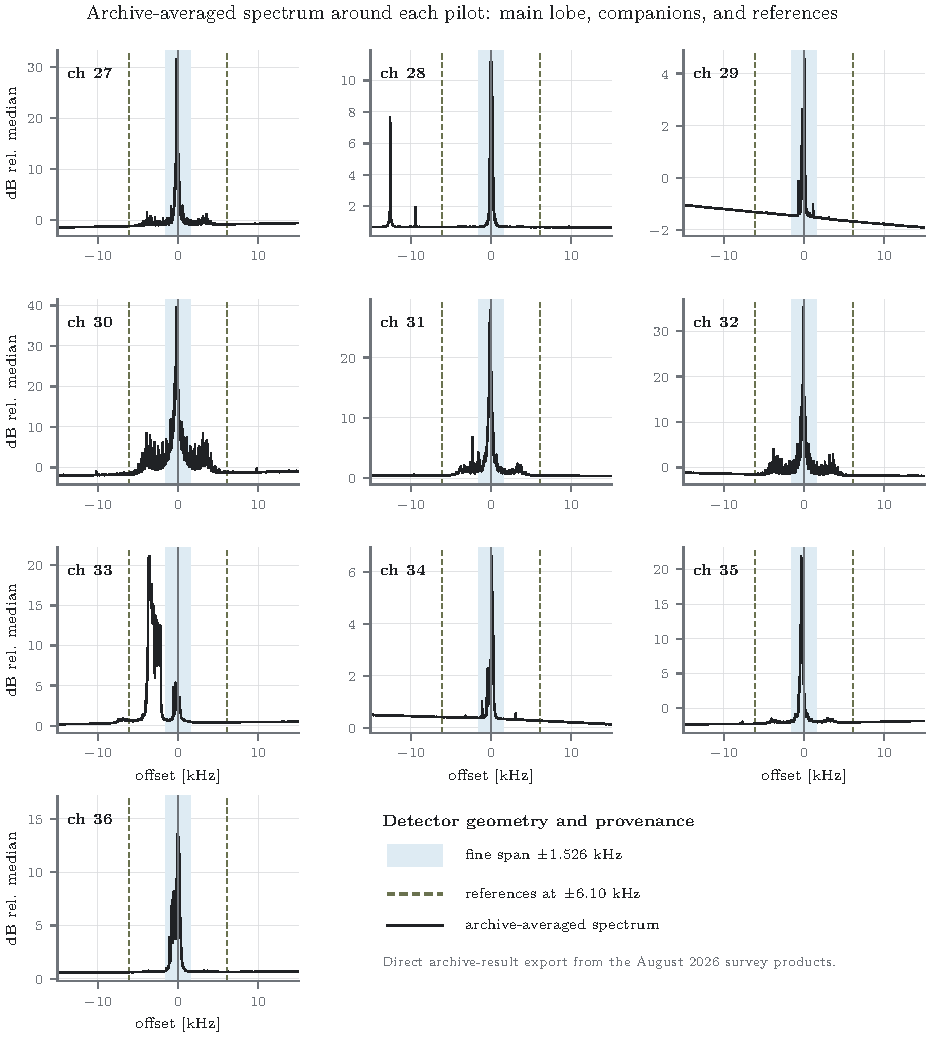
\includegraphics[height=0.70\textheight,width=0.98\linewidth,keepaspectratio]{figs/fig_census_psd.pdf}
\caption{The transmitter population's spectral face: archive-averaged spectrum within $\pm 15$~kHz of each pilot, from the survey products' stored integrated spectra (dB relative to the channel median). Shaded: the $K = 128$ fine span ($\pm 1.526$~kHz); dashed: the $\pm 2$-bin reference placements ($\pm 6.1$~kHz). Panels are centred on each channel's \emph{synthesized} (nominal) pilot in the transmitted-frequency sense, so a carrier's displacement from zero is its measured off-nominal offset. On eight of the ten channels the dominant carrier is a single compact lobe inside the fine span, within $0.4$~kHz of synthesis; on the crowded-field channels (30, 31, 32) it stands over the resolved sidelobe forest discussed in the text. Channel 33 is the documented exception: its dominant carrier sits at $-3.6$~kHz, in the skipped guard between the fine span and the lower reference, with companion structure near $-2.6$~kHz --- the off-nominal blind spot whose diagnostics Appendix~\ref{app:legacy} records. Channel 28's strongest in-window feature lies $12.6$~kHz below synthesis, far outside the capture geometry, while its nominal pilot stands at $11$~dB. The references sit in clean territory on every channel --- the placement validation of Section~\ref{sec:param:tradeoffs} made visually. The thirteen lower-band channels appear in Figure~\ref{fig:bao:lowerpsd}.}
\label{fig:census:psd}
\end{figure}

Two propagation mechanisms then modulate what the census delivers, and they are worth distinguishing carefully because they act on different timescales and different terms of the residual budget. \emph{Tropospheric ducting}: the radio refractive index of the lower atmosphere decreases with height, and when temperature inversions or sharp humidity gradients steepen that lapse past the critical value, a layer forms that refracts UHF energy back downward faster than the Earth curves away --- a waveguide along the surface \cite{itup453}. A ducted path delivers transmitters from hundreds of kilometers beyond the horizon at strengths that can rival line-of-sight, and the duct's formation and collapse follow the meteorology: evolution over tens of minutes to hours, organized diurnally and seasonally, and uncorrelated with the sidereal frame. \emph{Aircraft scatter}: an airframe is a moving bistatic reflector, and the scattered path carries a Doppler shift bounded by $2v/\lambda$ --- the same signals and Doppler scales that DTV-based passive radar exploits deliberately \cite{griffiths2017passive}. Table~\ref{tab:doppler} evaluates the bound by traffic class at the band's midpoint: the civil envelope tops out near $\pm 1$~kHz at jet cruise speed, inside the detector's fine span; military speeds exceed the span but are rare in this airspace; satellite forward scatter lands tens of kilohertz out --- far outside the capture window --- and transits in seconds. The observable signature is twofold: a frequency-smeared scattered component, and \emph{amplitude flutter} --- the beat between the direct and scattered paths at their Doppler difference, familiar from the analog era as ``airplane flutter'' --- with fading on timescales of seconds.

\begin{table}[t]
\centering
\caption{Maximum bistatic Doppler $2v/\lambda$ by reflector class, evaluated at the DTV band midpoint ($581$~MHz, $\lambda = 0.516$~m); values scale by $\pm 5\%$ across $554$--$608$~MHz. The civil-aircraft envelope sits inside the $\pm 1.526$~kHz fine span; satellite scatter lands far outside it and transits the beam in seconds, so its contribution is confined to the fast (sub-acquisition) share of the timescale decomposition.}
\label{tab:doppler}
\begin{tabular}{lcc}
\toprule
reflector class & typical speed & max Doppler \\
\midrule
light general aviation & $50$~m/s & $\pm 0.19$~kHz \\
turboprop / charter & $130$~m/s & $\pm 0.50$~kHz \\
commercial jet, cruise & $250$~m/s & $\pm 0.97$~kHz \\
military fast jet & $600$~m/s & $\pm 2.3$~kHz \\
satellite, low Earth orbit & $7.6$~km/s & $\pm 29$~kHz \\
\bottomrule
\end{tabular}
\end{table}

Neither mechanism is directly proven from the survey products, and this subsection does not claim to have separated them. What can be said is that they are separable in principle by timescale, and that the decomposition of Section~\ref{sec:bao:chain} already measures the relevant split: flutter's seconds-scale fading lands in the sub-acquisition (fast) share, which carries no coherence amplification and is benign; ducting's slow wander lands in the intra-day share, the term that carries $n_{\text{coh}}$ and dominates every failing budget. The measured structure --- intra-day shares that dominate the surviving power on most channels, and correlation times of $34$ and $45$ minutes where the estimator succeeds, timescales natural to duct evolution and impossible for flutter --- is circumstantial evidence that ducting is the principal slow modulator and Doppler flutter a fast-share contributor. A definitive attribution --- correlating shelf power against refractivity soundings, or the fine spectra against transponder-derived aircraft tracks --- is specified for the closing campaign rather than claimed here.

\section{Scope, Standard Evolution, \& Generalization}
\label{sec:dtv:scope}
The weight profiles of Chapter~\ref{sec:param} are specific to the A/53 standard: the implemented single-tone method detects the 8-VSB suppressed-carrier pilot and nothing else. Two boundaries of that scope should be stated explicitly. First, the broadcast standard itself is evolving. ATSC 3.0 replaces 8-VSB with an OFDM physical layer whose synchronization features --- a deterministic bootstrap preamble and embedded pilot subcarriers --- are structured differently, and the implemented single-tone profiles do not track that transition. The per-channel census and epoch structure of the survey accommodate a gradual transition naturally (a converted channel leaves the A/53 census), but detection of ATSC 3.0 emissions would require new profiles. Second, the method does not transfer geographically merely because the backend hardware does. An instrument sharing this digital signal chain but operating in a different regulatory domain --- HIRAX in South Africa, for example --- faces a different broadcast standard (DVB-T2, an OFDM system) on a different channel raster, so the weight bank is regulatory-domain data in the same sense that the calibration constants are channel data.

\textit{Porting to another receiver.} The constraint equations of
Chapters~\ref{sec:param} and \ref{sec:pipeline} are receiver-independent; the
numerical values are not, and it is worth being explicit about which is which,
because the natural assumption --- that a different telescope differs only by a
spectral-sense convention --- is wrong in a way that fails quietly. The sense
\emph{is} a convention, fixed per receiver profile, and a sense error announces
itself: the synthesized tone lands at the mirror frequency, the pilot is not
matched at all, and the channel simply never fires. What must be re-derived is
subtler. The coarse-channel rate $f_s$ sets the tap length through the census
requirement, since what that census fixes is the analysis window's width in
\emph{frequency}: a receiver whose raster is half as wide needs half the taps to
present the same window, and holding $K$ fixed instead silently halves both the
window and the unambiguous fine span. The frame length $N$ follows the
receiver's visibility-integration length, and with $K$ determines the sub-frame
count $L$ and hence which member of the transform family of
Section~\ref{sec:impl:fxfft} is required. The channel raster sets each pilot's
baseband offset $\delta\!f_c$ and normalized tone frequency $\nu_c$, so the
weight bank is regenerated per profile rather than transferred. The input count
$M$ enters the degrees of freedom that set the null width. Only the beacon
itself --- its existence, its standardized offset $\Delta f_{\text{pilot}}$, and
the shelf proxy relation of Eq.~\eqref{eq:shelfproxy} --- is a property of the
broadcast standard and carries over untouched.

The same observations define the method's generalization path. Nothing in the architecture is specific to a single sinusoidal beacon: the requirements on a detection feature are that it be standardized in frequency, spectrally concentrated or otherwise deterministic, and present whenever the transmitter radiates. OFDM broadcast standards satisfy these requirements through different structures --- continual pilot subcarriers at fixed carrier indices with known modulation, and repeated deterministic preambles --- and a generalized weight profile matched to a pilot comb rather than a single tone is the natural extension. This is not achievable in the current single-tone form, and it is left as future work; the framework of Chapters~\ref{sec:param}--\ref{sec:impl} (constraint-derived parameters, exact arithmetic, rank-based calibration against measured nulls) would carry over unchanged.
